\section{/home/aakash/mlpack/src/mlpack/core/util/arma\+\_\+config\+\_\+check.hpp File Reference}
\label{arma__config__check_8hpp}\index{/home/aakash/mlpack/src/mlpack/core/util/arma\+\_\+config\+\_\+check.\+hpp@{/home/aakash/mlpack/src/mlpack/core/util/arma\+\_\+config\+\_\+check.\+hpp}}
Include dependency graph for arma\+\_\+config\+\_\+check.\+hpp\+:
\nopagebreak
\begin{figure}[H]
\begin{center}
\leavevmode
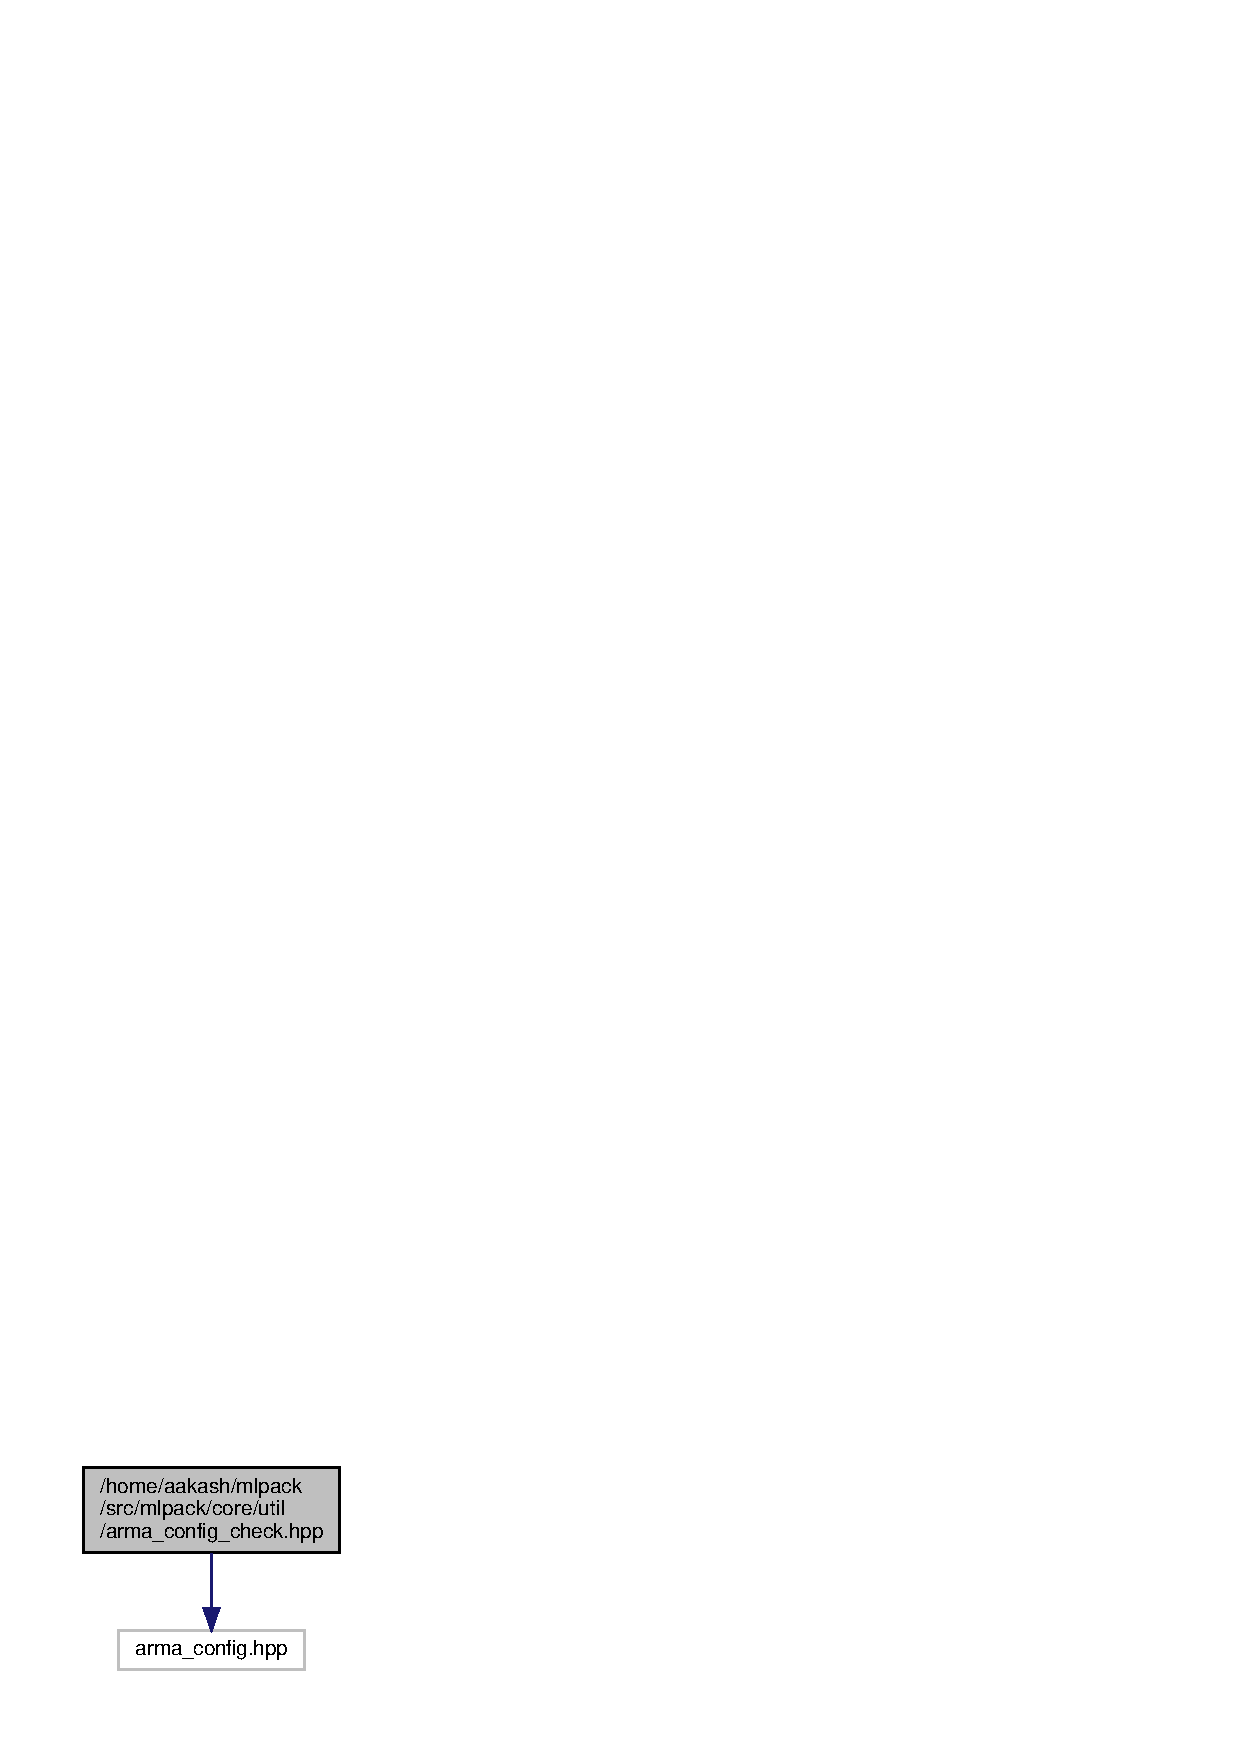
\includegraphics[width=167pt]{arma__config__check_8hpp__incl}
\end{center}
\end{figure}
This graph shows which files directly or indirectly include this file\+:
\nopagebreak
\begin{figure}[H]
\begin{center}
\leavevmode
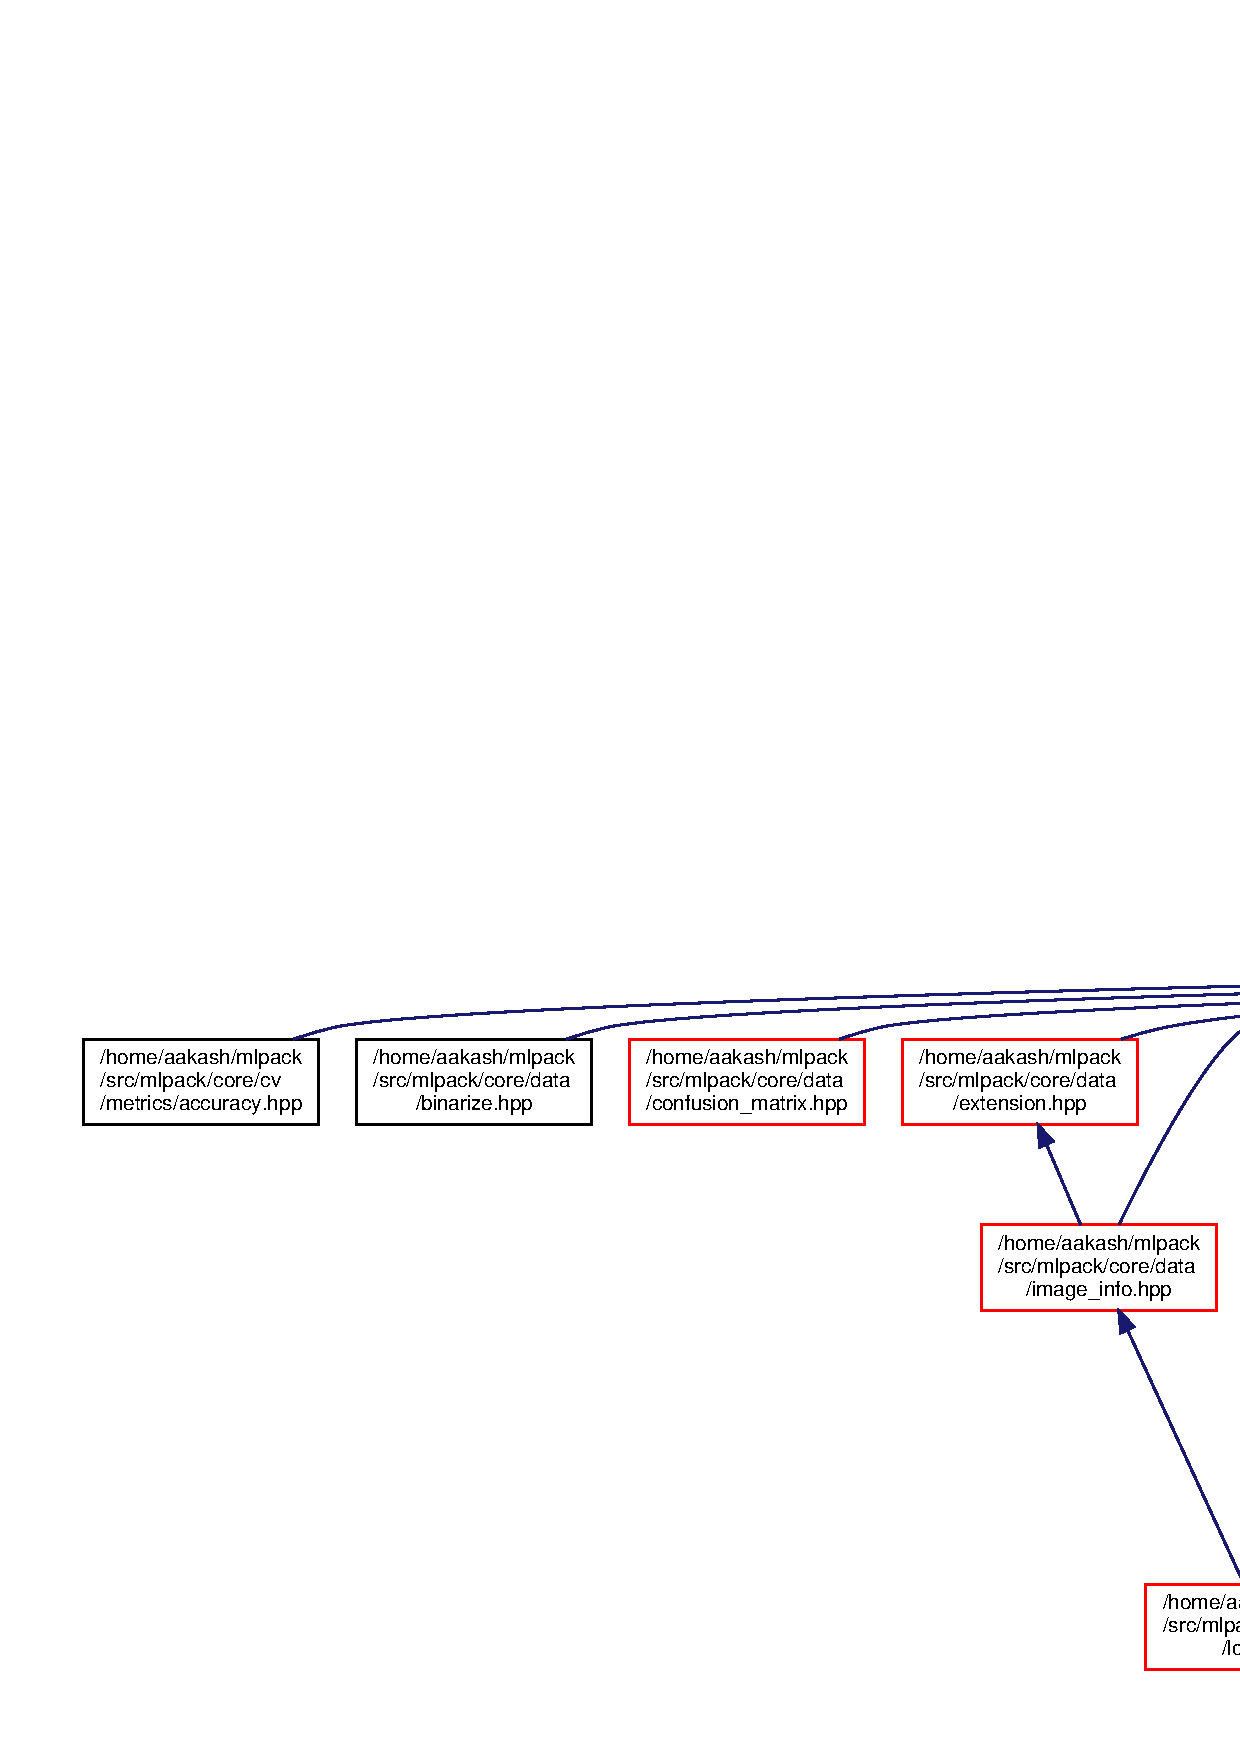
\includegraphics[width=350pt]{arma__config__check_8hpp__dep__incl}
\end{center}
\end{figure}


\subsection{Detailed Description}
\begin{DoxyAuthor}{Author}
Ryan Curtin
\end{DoxyAuthor}
Using the contents of arma\+\_\+config.\+hpp, try to catch the condition where the user has included mlpack with A\+R\+M\+A\+\_\+64\+B\+I\+T\+\_\+\+W\+O\+RD enabled but mlpack was compiled without A\+R\+M\+A\+\_\+64\+B\+I\+T\+\_\+\+W\+O\+RD enabled. This should help prevent a long, drawn-\/out debugging process where nobody can figure out why the stack is getting mangled.

mlpack is free software; you may redistribute it and/or modify it under the terms of the 3-\/clause B\+SD license. You should have received a copy of the 3-\/clause B\+SD license along with mlpack. If not, see {\tt http\+://www.\+opensource.\+org/licenses/\+B\+S\+D-\/3-\/\+Clause} for more information. 